\section{Dynamic Behavior Modeling}
All diagrams are numbered based on their section number.
\subsection{Complete Turn}
\begin{figure}[H]
   \centering
   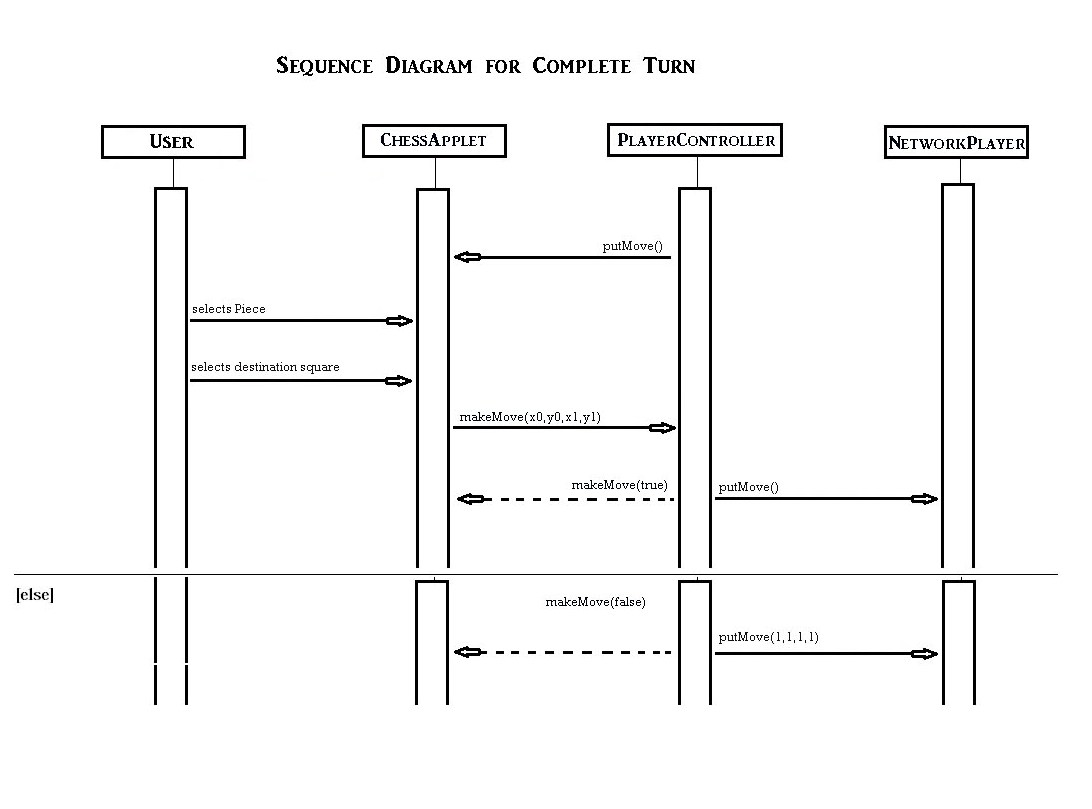
\includegraphics[scale=0.50]{seq_Complete_Turn.jpg}
   \caption{Sequence Diagram for Usecase Complete Turn}
  \end{figure}
  %\FloatBarrier
\subsection{Play Chess}
\begin{figure}[H]
   \centering
   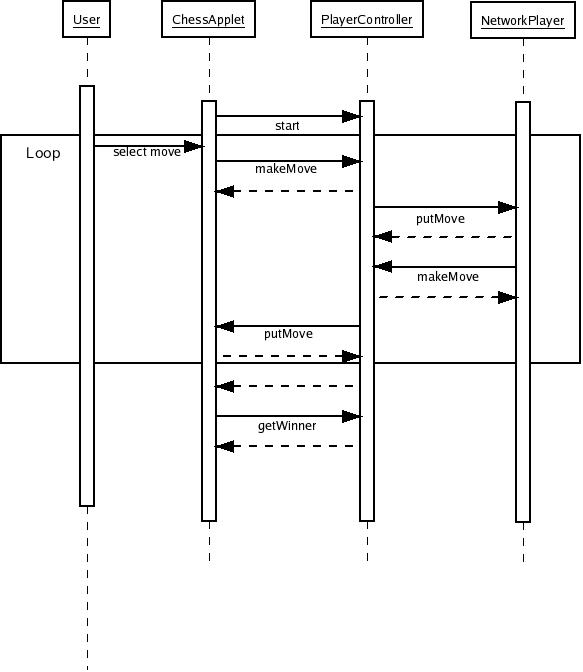
\includegraphics[scale=0.50]{seq_Play_Chess.jpg}
   \caption{Sequence Diagram for Usecase Play Chess}
  \end{figure}
  %\FloatBarrier
\subsection{Analyze Position}
\begin{figure}[H]
   \centering
   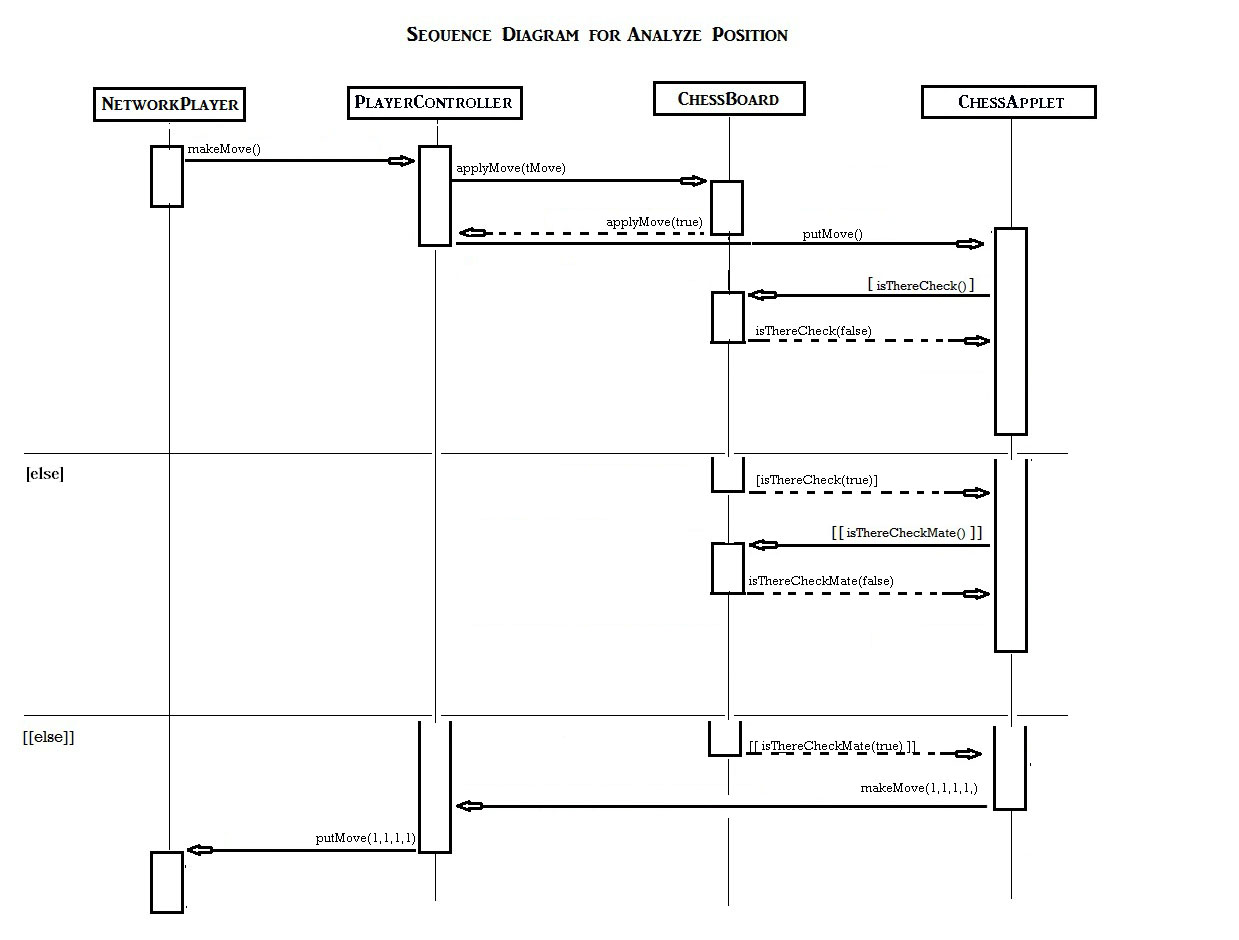
\includegraphics[scale=0.50]{seq_Analyze_Position2.jpg}
   \caption{Sequence Diagram for Usecase Analyze Position}
  \end{figure}
  %\FloatBarrier
\subsection{Quit Game}
\begin{figure}[H]
   \centering
   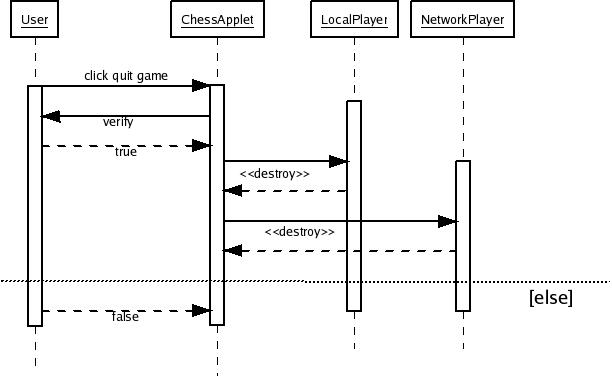
\includegraphics[scale=0.50]{seq_Quit_Game.jpg}
   \caption{Sequence Diagram for Usecase Quit Game}
  \end{figure}
  %\FloatBarrier
\subsection{Start Game}
\begin{figure}[H]
   \centering
   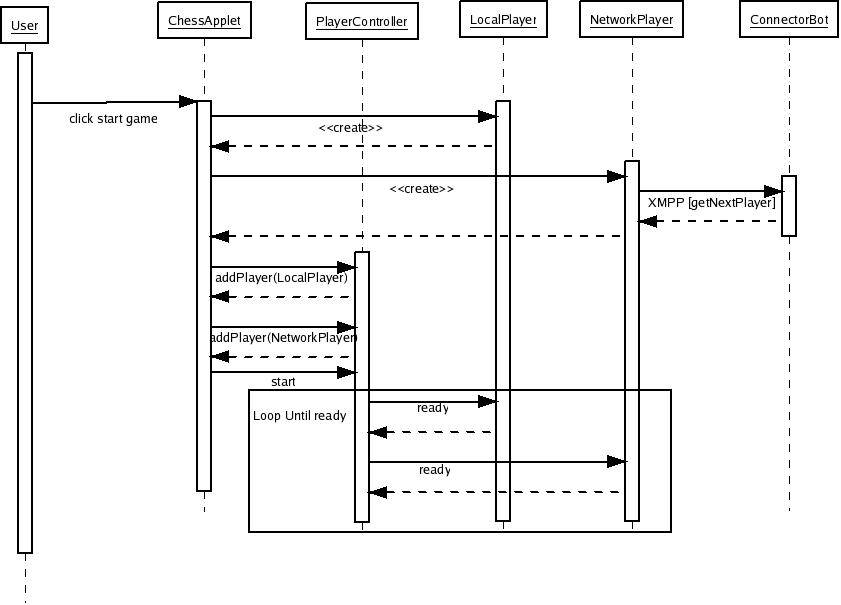
\includegraphics[scale=0.50]{seq_Start_Game.jpeg}
   \caption{Sequence Diagram for Usecase Start Game}
  \end{figure}
  %\FloatBarrier
\subsection{Validate Move}
\begin{figure}[H]
   \centering
   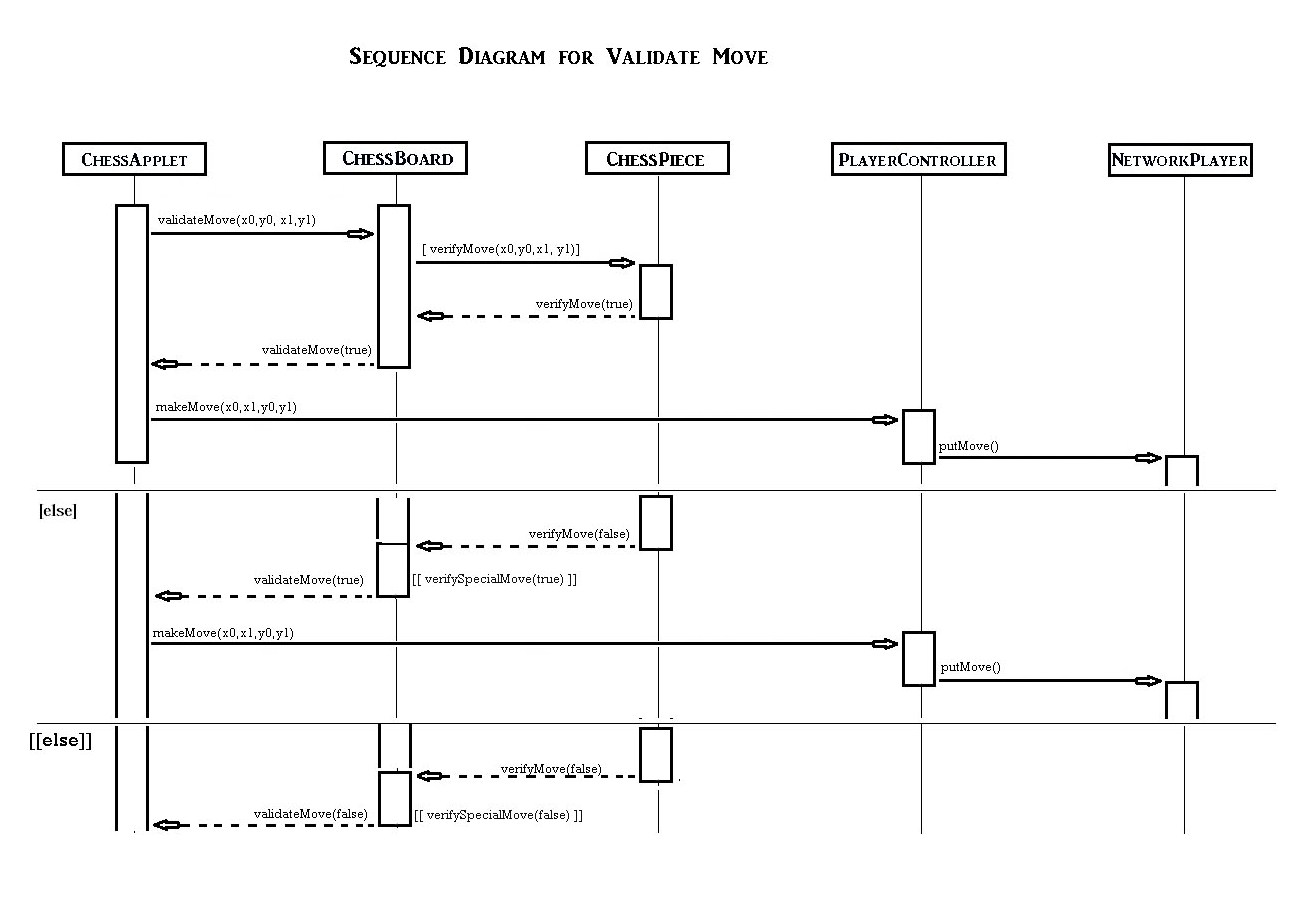
\includegraphics[scale=0.50]{seq_Validate_Move.jpg}
   \caption{Sequence Diagram for Usecase Validate Move}
  \end{figure}
  %\FloatBarrier
